\documentclass[letterpaper,twocolumn]{article}
\usepackage[top=3cm,bottom=2.5cm,hmargin=2.5cm]{geometry}
\usepackage{amsmath,amssymb,amsthm,mathtools}
%\usepackage{mathrsfs,bm,color}
\usepackage{hyperref,fancyhdr,lastpage}
%\usepackage{graphicx}
%\usepackage{tikz,tikz-cd}
%\usetikzlibrary{arrows,trees,positioning,shapes.geometric,shapes.misc}
\usepackage{caption}
\usepackage{subcaption}
\usepackage{algorithm}
\usepackage[noend]{algpseudocode}
%\usepackage{indentfirst}
\usepackage{lineno}
\usepackage{url}
\usepackage{appendix}
%\linenumbers

\pagestyle{fancy}
\renewcommand\headrule{}
\lhead{\today}
%\chead{adsf}
\rhead{Jeremy Ko}
\cfoot{\thepage}

\newtheorem{theorem}{Theorem}[]
\newtheorem{corollary}[theorem]{Corollary}
\newtheorem{lemma}[theorem]{Lemma}
\newtheorem{observation}[theorem]{Observation}
\newtheorem{definition}[theorem]{Definition}
\newtheorem{question}[theorem]{Question}

\algdef{SE}[SUBALG]{Indent}{EndIndent}{}{\algorithmicend\ }%
\algtext*{Indent}
\algtext*{EndIndent}

\bibliographystyle{plainurl}
\title{An Efficient Implementation of a Lock-free Binary Search Tree with Good Amortized Step Complexity}
\author{Jeremy Ko \\ Deparment of Computer Science, University of Toronto \\ jerko@cs.toronto.edu}
\date{}
\setcounter{tocdepth}{2} % Depth of table of contents 
\setcounter{secnumdepth}{3} % Depth in which sections are numbered

\newcommand{\flag}{\mathit{flag}}
\newcommand{\info}{\mathit{info}}
\newcommand{\code}[1]{\texttt{#1}}

\begin{document}
\maketitle

%\tableofcontents

\begin{abstract}
Lock-free data structures are those that may be queried and updated concurrently by multiple processes without the use of locks. In order to achieve lock-freedom, operations typically help other operations that must update the same part of the data structure. We give a new implementation of a lock-free binary search tree, called a $k$-lazy binary search tree (BST), using a lazy helping heuristic, in which for a fixed number of steps, processes do not perform any helping. We show a $k$-lazy BST has amortized step complexity $O(h + N)$, where $h$ is the height of the BST and $N$ is the number of processes in the system. In all scenarios tested, our $k$-lazy BST performs better than another lock-free BST with the same amortized step complexity.
\end{abstract}


\section{Introduction}

Lock-free data structures are an increasingly popular alternative to sequential data structures with the rise of multiprocessor computers. A \textit{lock-free data structure} allows operations to be performed concurrently by multiple processes, without the use of locks. Lock-free data structures are an attractive choice compared to lock-based data structures due to their performance and ability to withstand process failures. An implementation of a lock-free data structure guarantees that whenever there are active operations, some operation will eventually complete in a finite number of steps. Several implementations of lock-free data structures have been proposed, including those for linked lists~\cite{Valois95, Harris01, FomitchevR04}, doubly linked lists~\cite{Shafiei15}, binary search trees (BSTs)~\cite{EllenFRB10, EllenFHR13, Ko18}, and hash tables~\cite{Michael02, ShalevS06, PurcellH05}.

One way to compare the efficiency of various implementations of a data structure is to compare their worst-case step complexity. It is not possible to perform a worst-case analysis for lock-free data structures, since any particular operation may never complete. Instead, amortized analysis is used to give an upper bound on the worst-case number of steps performed during a sequence of data structure operations. An \textit{amortized data structure} is a lock-free data structure that is optimized for better amortized step complexity.

Unfortunately, amortized data structures are typically more complex and have more overhead when operations are performed without contention. For these reasons, these implementations may not actually perform well in practice compared to more simple lock-free data structures with worse amortized step complexity. This raises the question if there are more fine-grained analysis tools that can be used to better understand the complexity of lock-free data structures.

In this paper, we explore the performance of binary search trees with good amortized step complexity. We do this by proposing a new implementation of a BST, which we call a $k$-lazy BST. The implementation is divided two phases, a \textit{lazy phase} and a \textit{helping phase}. During the lazy phase, operations behave like a naive implementation of a BST that simply restarts whenever conflicts with other operations arise. If an operation does not complete within a constant amount of time, the operation enters the helping phase. During the helping phase, operations behave like an implementation of a lock-free BST with good amortized step complexity. Operations may be required to help other operations complete in order to guarantee lock-free progress. 
%Without the helping phase, our $k$-lazy BST will not guarantee lock-free progress.

We prove that our $k$-lazy BST has good amortized step complexity, and so performs well no matter how processes are scheduled or which operations are performed. In our experiments, we show that our $k$-lazy BST performs better than another implementation of a BST with the same amortized step complexity. For the workloads that were tested, our BST also outperforms a randomized skip list from the Java Concurrency Library.

The remainder of the paper is organized as follows. In Section~\ref{section_contribution}, we list our contributions. In Section~\ref{section_model}, we describe the asynchronous shared memory model. In Section~\ref{section_related}, we discuss prior implementations of lock-free BSTs and analysis techniques of lock-free data structures. In Section~\ref{section_implementation}, we describe the implementation of our $k$-lazy BST. In Section~\ref{section_results}, run experiments to compare our $k$-lazy BST against two other lock-free BSTs. In Section~\ref{section_conclusion}, we summarize our results and propose open problems.

\section{Contributions}\label{section_contribution}
In this paper, we make the following contributions:
\begin{enumerate}
	\item We discuss the limitations of current implementations of lock-free BSTs and the theoretical tools used to analyze them.
	\item We propose a new implementation of a lock-free binary search tree using a lazy helping heuristic, which we call a $k$-lazy BST. 
	\item We justify the correctness, progress guarantees, and amortized step complexity of our $k$-lazy BST.
	\item We show that our $k$-lazy BST performs better than other implementations of BSTs with the same amortized step complexity. We also show that our $k$-lazy BST performs better than the ConcurrentSkipListMap found in Java's Concurrency Library. 
\end{enumerate}

\section{Model}\label{section_model}

We use an asynchronous shared memory model with $N$ processes. Shared memory consists of a collection of shared variables accessible by all processes in the system. Processes access or modify shared variables using primitive instructions that are performed atomically: \textsc{Write}$(r, value)$, which stores $value$ into the shared variable $r$, \textsc{Read}$(r)$, which returns the value stored in $r$, and compare-and-swap (CAS)\index{CAS}. CAS$(r, old, new)$ compares the value stored in shared variable $r$ with the value $old$. If the two values are the same, the value stored in $r$ is replaced with the value $new$ and \textsc{True} is returned; otherwise \textsc{False} is returned. 

A \textit{configuration}\index{configuration} of a system consists of the values of all shared variables and the states of all processes. A \textit{step}\index{step} by a process either accesses or modifies a shared variable, and can also change the state of the process. An \textit{execution}\index{execution} is an alternating sequence of configurations and steps, starting with a configuration.  Given an execution, a \textit{scheduler} determines the next process to take a step, and the type of step taken by the process is determined by its algorithm. Processes may \textit{crash}, which means they no longer take steps following a certain configuration.

An operation on a data structure by a process becomes \textit{active}\index{active} when the process performs the first step of its algorithm. The operation becomes \textit{inactive}\index{inactive} after the last step of the algorithm is performed by the process. The \textit{execution interval}\index{execution interval} of the operation consists of all configurations in which it is active. In the initial configuration, the data structure is empty and there are no active operations. 

A lock-free data structure is considered to be correct if all executions of its operations are \textit{linearizable}~\cite{AttiyaW04}. An execution $\alpha$ is linearizable if one can assign linearization points to each completed operation and a subset of the uncompleted operations in $\alpha$ with the following properties. First, the linearization point of an operation is within its execution interval. Second, the return value of each operation in $\alpha$ must be the same as in the execution in which the same operations are performed atomically in order of their linearization points. 

The \textit{amortized step complexity}\index{amortized step complexity} of a data structure is the maximum number of steps in any execution consisting of operations on the data structure, divided by the number operations invoked in the execution. One can determine an upper bound on the amortized step complexity by assigning an \textit{amortized cost}\index{amortized cost} to each operation, such that for all possible executions $\alpha$ on the data structure, the total number of steps taken in $\alpha$ is at most the sum of the amortized costs of the operations in $\alpha$. The amortized cost of a concurrent operation is often expressed as a function of contention. For an operation $op$ in an execution, we define its \textit{point contention}, denoted $\dot{c}(op)$, to be the maximum number of active operations in a single configuration during the execution interval of $op$. 

\section{Related Work}\label{section_related}

\subsection{On the Limitations of Theoretical Analysis Tools}
Many lock-free data structures have been design with varying amortized step complexity. Ellen, Fatourou, Ruppert, and van Breugel gave an implementation of lock-free binary search tree~\cite{EllenFRB10}, which we call a EFRB-BST. It has $\Omega(h(op)\dot{c}(op))$ amortized step complexity, where $h(op)$ is the height of the BST at the start of an operation $op$ and $\dot{c}(op)$ is the point contention of $op$. 

Ellen, Fatourou, Helga, and Ruppert give a different implementation of a BST, which we call a EFHR-BST, that has $O(h(op) + \dot{c}(op))$ amortized step complexity~\cite{EllenFHR13}. We will describe this implementation in detail in the next section. Even though this implementation has better amortized step complexity, it is more complex and has more overhead when operations are performed without contention. For these reasons, this implementation may not actually perform well in practice. Furthermore, its use of helping also causes unnecessary write contention. This means that it creates executions in which all $N$ processes in the system may be collectively working to help complete a single operation. Gibson and Gramoli~\cite{GibsonG15} have proposed that operations should aim to avoid helping as much as possible. 

Some recent works aim to prove that the worst-case executions of lock-free data structures do not occur often. Alistarh et al. analyze the expected runtime of simple lock-free data structures assuming an \textit{uniform stochastic scheduler}~\cite{AlistarhCS14}. In this model, the next process to take a step chosen by the scheduler is decided uniformly at random. For a class of lock-free data structures, which they call \textit{single compare-and-swap universal} (SCU), they prove that the expected number of steps to complete a single operation is $O(\sqrt{N})$, where $N$ is the number of processes in the system. Unfortunately, most practical lock-free data structures, such as the BSTs mentioned previously, are not in the class SCU. It is not clear how to extend their complicated analysis to apply to these data structures. Furthermore, their assumption of an uniform stochastic scheduler does not seem to be a realistic representation of real operating system process schedulers.

\subsection{A Previous Implementation of Binary Search Tree}\label{section_bst_EFHR}
Our new $k$-lazy BST is based heavily on a EFHR-BST. In this section, we give a high-level description of the implementation of the EFHR-BST. 

The BST implements a dynamic set $S$ of keys, supporting the operations \textsc{Insert}$(x)$, \textsc{Delete}$(x)$, and \textsc{Search}$(x)$. The binary search tree is \textit{leaf-oriented}, so every key in the dynamic set corresponds to a leaf and all nodes have 0 or 2 children. Internal nodes are only used to direct searches to a leaf. This implementation uses the concepts of \textit{flagging} and \textit{marking}. Each node contains a flag bit, which is used to signify that an \textsc{Insert} or \textsc{Delete} operation is attempting to perform an update at one of the node's children. Each node also contains a marked bit, which signifies that it will be removed from the BST. Before a node is removed from the BST, it must be marked. Once a node becomes marked, it is never unmarked. Each node contains an $\info$ pointer to an \textsc{UpdateRecord}, which stores information about a particular update operation that is used to allow processes to complete an update operation on another's behalf. When a node is flagged or marked by an operation, its is also updated to point to the \textsc{UpdateRecord} of the current operation. The flag bit, mark bit, and $\info$ pointer of each node are stored in a single field so that they can be updated simultaneously by a single CAS.

A new node can be inserted into the binary search tree by replacing a leaf $l$ with a new subtree of three nodes. This is done by a series of three CAS instructions on the parent, $p$, of $l$, performing the following actions: 1) flagging $p$, 2) updating a child pointer of $p$ to point to the new subtree, and 3) unflagging $p$. This is illustrated in Figure~\ref{fig_bst_insert}. 

\begin{figure*}[!tb]
	\centering
	\begin{subfigure}[b]{0.3\textwidth}\centering
		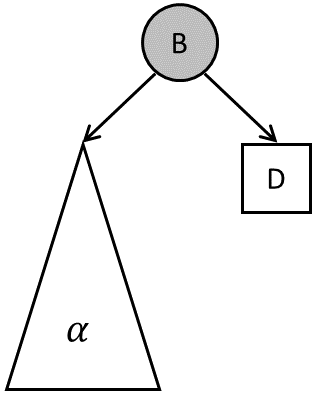
\includegraphics[width=0.5\textwidth]{bst_ins_2.png} % 740 px
		\caption{Flag B}
	\end{subfigure}
	\quad
	\begin{subfigure}[b]{0.3\textwidth}\centering
		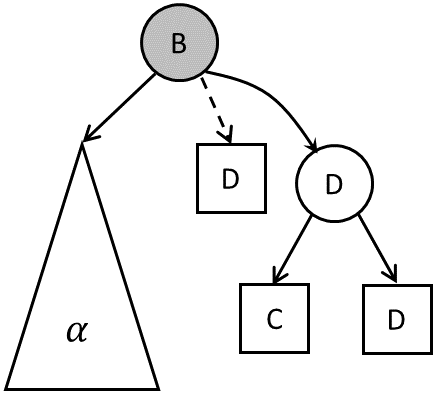
\includegraphics[width=0.7\textwidth]{bst_ins_3.png} % 740 px
		\caption{Update B's child}
	\end{subfigure}
	\quad
	\begin{subfigure}[b]{0.3\textwidth}\centering
		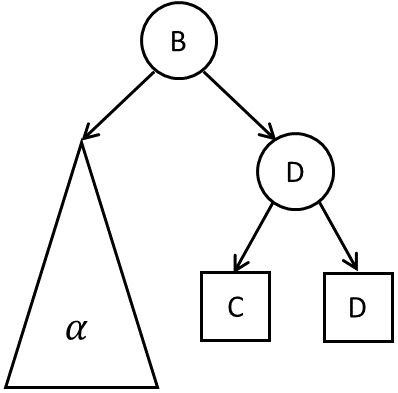
\includegraphics[width=0.65\textwidth]{bst_ins_4.png} % 740 px
		\caption{Unflag B}
	\end{subfigure}
	\caption{The steps to perform \textsc{Insert}(C). Flagged nodes are gray and marked nodes are crossed.}\label{fig_bst_insert}
\end{figure*}

A node $l$, as well as its parent, can be removed from the binary search tree by updating the child pointer of $l$'s grandparent to point to $l$'s sibling. This is done by a series of four CAS instructions performing the following actions: 1) flagging $l$'s grandparent, $gp$, 2) marking $l$'s parent, $p$, 3) updating a child pointer of $gp$ to point to $l$'s sibling, and 4) unflagging $gp$. This is illustrated in Figure~\ref{fig_bst_delete}.

%CAS instructions that attempt to change the state of a node from \textsc{Clean} to either \textsc{IFlag} or \textsc{DFlag} are called \textit{flagging} CAS. CAS instructions that attempt to change the state of a node from \textsc{Clean} to \textsc{Mark} are called \textit{marking} CAS. 
\begin{figure*}[!bt]
	\centering
	\begin{subfigure}[b]{0.2\textwidth}\centering
		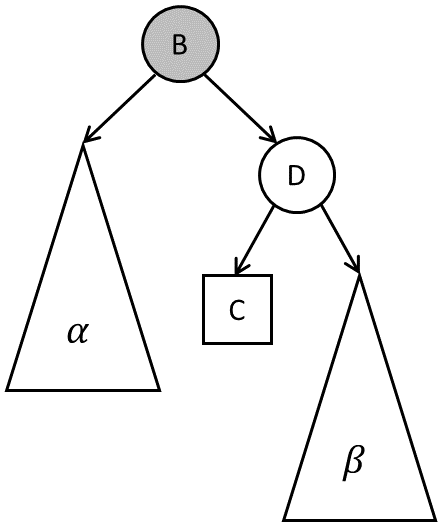
\includegraphics[width=1\textwidth]{bst_del_2.png}
		\caption{Flag B}
	\end{subfigure}
	\qquad
	\begin{subfigure}[b]{0.2\textwidth}\centering
		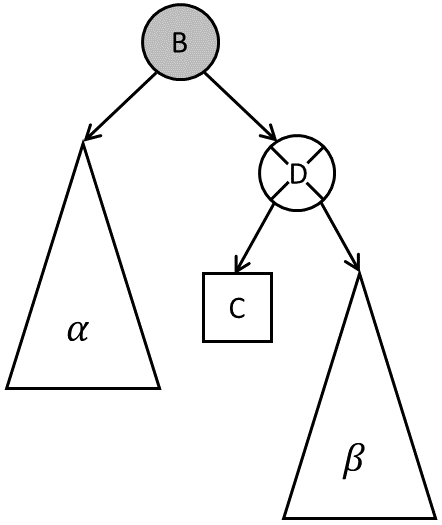
\includegraphics[width=1\textwidth]{bst_del_3.png} 
		\caption{Mark D}
	\end{subfigure}
	\qquad
	\begin{subfigure}[b]{0.2\textwidth}\centering
		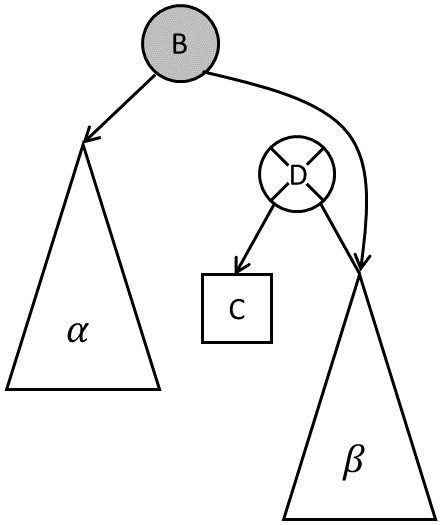
\includegraphics[width=1\textwidth]{bst_del_4.png} 
		\caption{Update B's child}
	\end{subfigure}
	\qquad
	\begin{subfigure}[b]{0.2\textwidth}\centering
		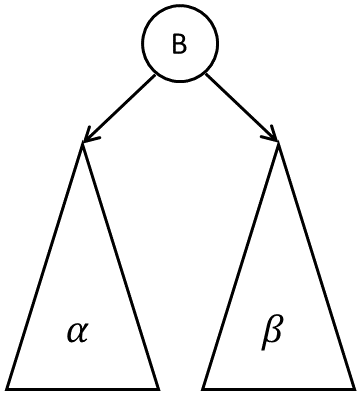
\includegraphics[width=0.85\textwidth]{bst_del_5.png} 
		\caption{Unflag B}
	\end{subfigure}
	\caption{The steps to perform \textsc{Delete}(C). Flagged nodes are gray and marked nodes are crossed.}\label{fig_bst_delete}
\end{figure*}

Consider a successful \textsc{Insert}$(x)$ or \textsc{Delete}$(x)$ operation $op$ that modifies the binary search tree. The operation is divided into a series of \textit{update attempts}. The first attempt of $op$ begins by searching for the key $x$ starting from the root of the binary search tree until a leaf is found, and then performing the appropriate series of CAS instructions mentioned previously. These CAS instructions may be unsuccessful if there are concurrent operations modifying the same nodes. For example, the flagging CAS by $op$ that attempts to flags a node $p$ may be unsuccessful because $p$ has been previously flagged or marked by a different operation $op'$. When such a conflict occurs, $op$ \textit{helps} the operation that previously flagged or marked $p$ to complete by using the \textsc{UpdateRecord} pointed to by $p.\info$. If $op$ is helping an \textsc{Insert} operation $op'$, $op'$ is guaranteed to be completed in its current attempt (either by itself or by a helping operation). Once completed, $op$ starts a new attempt. If $op$ helps an \textsc{Delete} operation $op'$, $op'$ may be unable to complete if $op'$'s marking CAS is unsuccessful. In this case, a \textit{backoff CAS} for $op'$ is performed, which unflags the node that is flagged for $op'$. At this point, $op'$ is no longer preventing $op$ from completing, so $op$ starts a new attempt.

When a new attempt begins, $op$ can simply repeat its steps, beginning with a search starting from the root. Instead, the implementation uses the concept of backtracking. Each process maintain a local stacks of node pointers. Each time a node is visited during a search, the process performing $op$ pushes a pointer to the node onto its local stack. Attempts by $op$ after its first attempt can be restarted by popping nodes off its stack until an unmarked node $m$ is found. Instead of performing a search from the root, $op$ can perform a search starting from $m$. It is proven that $m$ is a node that $op$ would visit during a solo execution of a search starting from the root of the binary search tree.


\section{The Implementation of a $k$-Lazy BST}\label{section_implementation}
As discussed in Section~\ref{section_related}, the BST implementation by Fomitchev and Ruppert has high overhead compared to other BSTs with worse amortized step complexity. Our new BST, which we call a $k$-lazy BST, aims to reduce this overhead by performing several attempts without helping. Only after a sufficient number of unsuccessful attempts have occurred should operations perform extra overhead to guarantee progress. The idea is that in real systems, an operation does not block another operation from completing for a long period of time. By the time an operation restarts a new insert or delete attempt, the blocking operation $op'$ has hopefully completed its own operation by itself. 

We next describe our $k$-lazy BST, where $k$ is a small constant. Each update operation, either \textsc{Insert}$(x)$ or \textsc{Delete}$(x)$, is divided into lazy phase and a helping phase. Both phases are divided into a series of attempts. Intuitively, our $k$-lazy BST will perform $k$ lazy attempts in which it attempts to complete the operation without performing any helping steps. If the operation is not successful within these $k$ lazy attempts, the operation enters the helping phase in which it behaves exactly like the \textsc{Insert} and \textsc{Delete} operations from EFRB-BST.

We first describe our algorithm for an \textsc{Insert}$(x)$ operation $op$ in more detail. All attempts of the lazy phase begin with a search through the BST for the key $x$ starting at the root. If a node with key $x$ is found, the operation returns. So suppose no node with key $x$ is found, and let $B$ be the parent node of the insertion point of $op$. A new update record $R_{op}$ is created for $op$. A flagging CAS is performed at $B$, which attempts to update $B$'s $\info$ pointer to point to $R_{op}$. If the flagging CAS is successful, $op$ proceeds to complete the insertion transformation as described in Section~\ref{section_bst_EFHR}. No other operation can prevent $op$ from completing once the flagging CAS is successful. If the flagging CAS is unsuccessful, then a new lazy attempt is started. If the insertion is not successful after $k$ attempts, $op$ enters the helping phase. At the start of the helping phase, an new local stack is initialized for $op$. We use this stack to proceed with the \textsc{Insert}$(x)$ operation from EFRB-BST until successful.

Our algorithm for a \textsc{Delete}$(x)$ operation $op$ follows similarly. In each lazy attempt of $op$, $op$ begins with a search through the BST for the key $x$ starting at the root. Assuming a leaf $\ell$ with key $x$ is found, $op$ attempts to remove $\ell$ from the BST using the deletion transformation outlined in Section~\ref{section_bst_EFHR}. If the flagging or marking CAS of $op$ is unsuccessful, $op$ unflags any nodes that were flagged for $op$, and then begins a new lazy attempt. After $k$ unsuccessful lazy attempts, $op$ enters the helping phase, in which it performs the \textsc{Delete}$(x)$ operation from EFRB-BST.

Our $k$-lazy BST implementation is linearizable. Intuitively, this is because the steps to perform updates to the BST are done exactly as in the EFRB-BST, which is a linearizable implementation of a BST. The at most $k$ lazy attempts of our implementation can only affect its step complexity. In the following theorem, we give an amortized analysis of our $k$-lazy BST, showing it has the same amortized step complexity as the EFRB-BST.

\begin{theorem}
For any finite $k \geq 0$, the amortized cost of \textsc{Insert}, \textsc{Delete}, and \textsc{Search} operations $op$ of a $k$-lazy BST is $O(h(op) + \dot{c}(op))$.
\end{theorem}

\begin{proof}
For any finite execution $\alpha$, the total number of steps taken during the helping phases of operations is bounded above by
\begin{equation*}
\sum_{op\in\alpha} helpingSteps(op) = O\bigg(\sum_{op\in\alpha} (h(op) + \dot{c}(op))\bigg).
\end{equation*}
This follows directly from the amortized step complexity of an EFRB-BST. 

We must therefore give a bound on the total number of steps taken during the lazy phases. We count the total number of steps taken during searches using a charging scheme.  Each attempt of the lazy phase of an operation $op$ performs a search starting from the root. If a node $x$ visited during the search is in the BST at the start of $op$, charge the node traversal to $op$. By definition, there are at most $h(op)$ such nodes charged to $op$ each lazy attempt. So suppose $x$ was added to the BST by a concurrent operation $op'$ sometime after the start of $op$. We charge the traversal of $x$ to $op'$. Since $op$ performs at most 1 insert or delete transformation (not including the modifications it makes to the BST during helping), each of which adds at most 2 new nodes onto a single path in the tree, $O(\dot{c}(op))$ node traversals are charged to $op$ by other operations in a single attempt. Each lazy attempt performs a constant number of steps that are not node traversals, such as the flagging, marking, and unflagging CASs. Since $op$ performs at most $k$ lazy attempts, it follows that
\begin{equation*}
\sum_{op\in\alpha} lazySteps(op) = O\bigg(\sum_{op\in\alpha} k(h(op) + \dot{c}(op))\bigg).
\end{equation*}

The total number of steps taken by an operation $op$ is $steps(op) = helpingSteps(op) + lazySteps(op)$. Therefore, for any finite $k \geq 0$,
\begin{equation*}
\sum_{op\in\alpha} steps(op) = O\bigg(\sum_{op\in\alpha} (h(op) + \dot{c}(op))\bigg).
\end{equation*}
\end{proof}

The amortized step complexity of a $k$-lazy BST implies that the BST is lock-free.
\begin{corollary}
For any finite $k \geq 0$, a $k$-lazy BST is lock-free.
\end{corollary}

\section{Results}\label{section_results}
In this section, we compare the throughput (operations per second) of our $k$-lazy BST against other lock-free dynamic set implementations in various experiments.

\begin{figure*}[!tb]
	\centering
	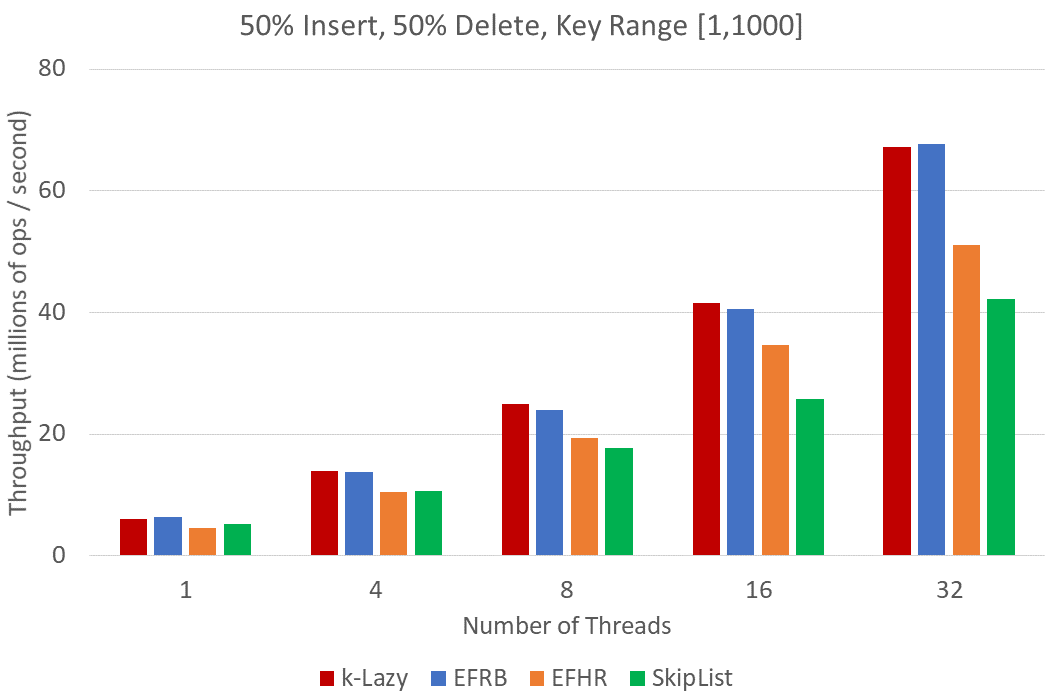
\includegraphics[width=0.80\textwidth]{results.png} 
	\caption{The throughput (in millions of operations per second) of a $k$-lazy BST EFRB-BST, EFHR-BST, and ConcurrentSkipListMap for a varying number of threads.}
	\label{results}
\end{figure*}


\subsection{Experimental Setup}
Brown has provided an implementation of the EFRB-BST in Java as well as a framework for testing concurrent data structures~\cite{BrownImpl19}. There is no implementation of the EFHR-BST. Brown's implementation of the EFRB-BST was used as a starting point to develop an implementation of both an EFRB-BST and $k$-lazy BST. The parameter $k$ for our $k$-lazy BST implementation was set to $k = 5$. The source code of our implementations can be found at \url{https://github.com/Jer-kO/csc2222-project}. Note that there is no implementation of a lock-free BST in the Java Concurrency Library. Thus, we compare our $k$-lazy BST against Java's ConcurrentSkipListMap.

All experiments were run on an m5d.8xlarge Amazon EC2 instance, with 32 virtual CPUs. In each experiment, each thread in a system of size $N \in  \{1, 4, 8, 16, 32\}$ is scheduled to perform as many data structure operations as possible in a 30 second time frame. The type of operation performed by each processes is chosen randomly, with 50\% of the operations being \textsc{Insert} and 50\% being \textsc{Delete}. The key of each operation is chosen uniformly at random in the range between 0 to 1000. In order to maximize the number of conflicting updates, the key range was kept small and no \textsc{Search} operations were performed. The algorithms to perform \textsc{Search} operations are the same in all 3 BST implementations considered, and so were not tested. Throughput is calculated by dividing the total number of operations completed by all threads in the system by the running time of the experiment. Each experiment was repeated for 3 trials, and the throughput reported is the average of the 3 trials. Figure~\ref{results} summarizes the results of our experiments.

\subsection{Discussion of Results}
In all experiments, the $k$-lazy BST performs as well as the EFRB-BST. Notice that the EFHR-BST which has amortized step complexity $O(h(op) + \dot{c}(op))$ performs worse than the EFRB-BST, which has amortized step complexity $\Omega(h(op)\dot{c}(op))$. However, all 3 lock-free BST implementations before better than the concurrent skip list provided by Java's Concurrency Library. 

We suspect that the EFHR-BST does not perform as well as the EFBR-BST or $k$-lazy BST due to the overhead of performing stack operations. The majority of operations complete after a single attempt, and so there is little advantage in backtracking. Finding an operation workload in which the advantages of an EFHR-BST can be observed is difficult. When keys are inserted uniformly at random in the range $[0,M]$, it can be shown that with high probability, the resulting tree has height $\Theta(\log M)$~\cite{CLRS}. Thus, we require a large key range so that restarting searches from the root is expensive compared to backtracking from a leaf. However, when the key range is large, the probability that we observe conflicting updates is small. With $N$ threads, the probability of scheduling an operation  that conflicts with another thread is less than $N/M$. Thus, if most operations complete within their first attempt, storing all nodes in a local stack is again useless. In applications that generate unbalanced BSTs with many overlapping update operations, we suspect that the EFHR-BST to perform better than a EFBR-BST. 

Due to time constraints, we do not provide results for any other operation workloads. Different \textsc{Insert} to \textsc{Delete} ratios and key ranges can easily be tested by the testing framework. Initial tests of such changes does not show any drastic differences in the reported throughput.

\section{Conclusion}\label{section_conclusion}
We have given an new implementation of a lock-free binary search tree, called a $k$-lazy BST, which has amortized step complexity $O(h(op) + \dot{c}(op))$.

There are several open problems and directions for future research. First, we observe that operation that enter the helping phase of a $k$-lazy BST and all update operations for a EFHR-BST require $\Theta(h(op))$ extra space to store all nodes visited during searches onto a local stack. We ask if it is possible to implement a lock-free BST with $O(h(op) + \dot{c}(op))$ amortized step complexity using $o(h(op))$ extra space per process.

There are a few implementations of lock-free balanced binary search trees~\cite{BrownER14}. One such implementation has good amortized step complexity~\cite{Ko18}. It will be interesting to see if the concept of dividing operations into a lazy phase and helping phase can be extended to balanced BSTs.

Finally, we ask if there are better theoretical or experimental tools to analyze lock-free data structures. This paper has shown the limitations of current theoretical and experimental tools. The goal of such research is to be able to suggest an efficient lock-free data structure for any given application.

\section{Acknowledgments}
I would like to thank Maryam Mehri Dehnavi for her helpful feedback.

%\nocite{*}
\bibliography{sources}

\onecolumn
\appendix
\appendixpage
\section{Reproducibility Appendix}

Experiments were run on an m5d.8xlarge Amazon EC2 instance, with 32 virtual CPUs. The implementations of the $k$-lazy BST, EFBR-BST, and EFHR-BST can be cloned from the following git repository \url{https://github.com/Jer-kO/csc2222-project}:
\begin{center}
\code{git clone git@github.com:Jer-kO/csc2222-project.git}
\end{center}

\noindent The following Java 8 version was installed:
\begin{center}
	\code{sudo yum install java-1.8.0-openjdk-devel}
\end{center}

\noindent The source code can be compiled into a bin folder using \texttt{javac}:
\begin{center}
\code{javac -d bin/ -cp src src/main/Main.java}
\end{center}

When running the testing framework, the first four input arguments specify the number of threads, number of trials, number of seconds per trial, and the type of algorithm to test, respectively. The type of algorithm must be one of \{``KLazy'', ``EFBR'', ``EFHR'', ``SkipList''\}. The percentage of \textsc{Insest} and \textsc{Delete} operations is specified using the \texttt{-ins\#} and \texttt{-del\#} options. The remainder of the operations are \textsc{Search} operations. The key range is specified with the \texttt{-keys\#} option. Finally, the output file containing the results is specified with the \texttt{-file\#} option.

For example, running the command
\begin{center}
	\code{java -cp bin main.Main 32 3 30 KLazy -ins50 -del50 -keys1000 -file-klazy4\_50\_50\_1000.csv}
\end{center}
runs an experiment with 32 threads, 3 trials, 30 seconds per trial, on the $k$-lazy BST with a 50\%-50\% \textsc{Insert} to \textsc{Delete} ratio on a key range of $[0,1000]$. Results of all trials are recorded in a new file called \texttt{klazy4\_50\_50\_1000.csv}. In particular, the file contains a column labeled \texttt{throughput}, which was used to generate all results reported in this paper. The reported throughput was the average of all trials.

\end{document}

